\begin{problem}{Bayes' Nets Representation}


\begin{question}[]{\bf Graph structure: Representational Power}

Recall that any directed acyclic graph $G$ has an associated family of probability
distributions, which consists of all probability distributions that
can be represented by a Bayes' net with structure $G$.

For the following questions, consider the following six directed
acyclic graphs:

\begin{center}
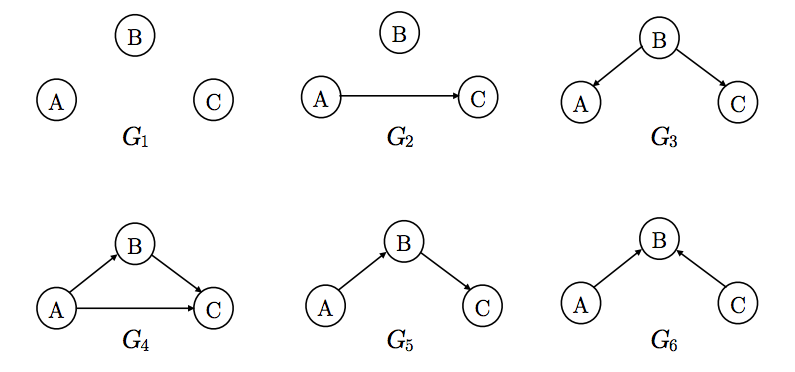
\includegraphics[height=3in]{figures/bayes_nets}
\end{center}

\begin{subquestion}[6]
Assume all we know about the joint distribution $P(A,B,C)$ is that it
can be represented by the product $P(A|B,C) P(B|C) P(C)$.  Mark each
graph for which the associated family of probability distributions is
guaranteed to include $P(A, B, C)$.

\begin{table}[h!]
\hfill
\begin{tabular}{ p{1.5in} p{1.5in} p{1.5in} }
\OneAi
\end{tabular}
\hfill
\end{table}
\end{subquestion}

\vspace{0.5in}

\begin{subquestion}[6]
Now assume all we know about the joint distribution $P(A,B,C)$ is that it
can be represented by the product $P(C|B) P(B|A) P(A)$.  Mark each
graph for which the associated family of probability distributions is
guaranteed to include $P(A, B, C)$.


\begin{table}[h!]
\hfill
\begin{tabular}{ p{1.5in} p{1.5in} p{1.5in} }
\OneAii
\end{tabular}
\hfill
\end{table}
\end{subquestion}

\end{question}

\newpage
\begin{question}[]{\bf Marginalization and Conditioning}

Consider a  Bayes' net over the random variables $A, B, C, D, E$ with
the structure shown below, with full joint distribution $P(A,B,C,D,E)$.

The following three questions describe different, unrelated situations (your answers to one question should not influence your answer to other questions).


\begin{figure}[h!]
\centering
  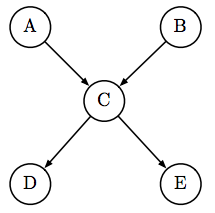
\includegraphics[height=1.5in]{figures/bayes_marg_q1}
\end{figure}

\begin{subquestion}[6]
Consider the marginal distribution $P(A, B, D, E) = \sum_c P(A, B, c, D, E)$,
where $C$ was eliminated.
On the diagram below, draw the minimal number of arrows that results
in a Bayes' net structure that is able to represent this marginal
distribution.  If no arrows are needed write ``No arrows needed.'' \\

\begin{minipage}[c]{\linewidth}
    \centering
    \OneBi
    \vspace{.25in}
  \end{minipage}

\end{subquestion}

\begin{subquestion}[6]
Assume we are given an observation: $A=a$.
On the diagram below, draw the minimal number of arrows that results
in a Bayes' net structure that is able to represent the conditional distribution $P(B,C,D,E \mid A=a)$.
 If no arrows are needed write ``No arrows needed.'' \\

\begin{minipage}[c]{\linewidth}
    \centering
    \OneBii
    \vspace{.25in}
  \end{minipage}
\end{subquestion}

\begin{subquestion}[6]
Assume we are given two observations: $D=d, E=e$.
On the diagram below, draw the minimal number of arrows that results
in a Bayes' net structure that is able to represent the conditional distribution $P(A,B,C \mid D=d, E=e)$.
 If no arrows are needed write ``No arrows needed.''
\begin{minipage}[c]{\linewidth}
    \centering
    \OneBiii
    \vspace{.25in}
  \end{minipage}
\end{subquestion}

\end{question}

\end{problem}